%\documentclass[journal]{vgtc}                % final (journal style)
\documentclass[review,journal]{vgtc}         % review (journal style)
%\documentclass[widereview]{vgtc}             % wide-spaced review
%\documentclass[preprint,journal]{vgtc}       % preprint (journal style)

%% Uncomment one of the lines above depending on where your paper is
%% in the conference process. ``review'' and ``widereview'' are for review
%% submission, ``preprint'' is for pre-publication, and the final version
%% doesn't use a specific qualifier.

%% Please use one of the ``review'' options in combination with the
%% assigned online id (see below) ONLY if your paper uses a double blind
%% review process. Some conferences, like IEEE Vis and InfoVis, have NOT
%% in the past.

%% Please note that the use of figures other than the optional teaser is not permitted on the first page
%% of the journal version.  Figures should begin on the second page and be
%% in CMYK or Grey scale format, otherwise, colour shifting may occur
%% during the printing process.  Papers submitted with figures other than the optional teaser on the
%% first page will be refused. Also, the teaser figure should only have the
%% width of the abstract as the template enforces it.

%% These few lines make a distinction between latex and pdflatex calls and they
%% bring in essential packages for graphics and font handling.
%% Note that due to the \DeclareGraphicsExtensions{} call it is no longer necessary
%% to provide the the path and extension of a graphics file:
%% 
\includegraphics{diamondrule} is completely sufficient.
%%
\ifpdf%                                % if we use pdflatex
  \pdfoutput=1\relax                   % create PDFs from pdfLaTeX
  \pdfcompresslevel=9                  % PDF Compression
  \pdfoptionpdfminorversion=7          % create PDF 1.7
  \ExecuteOptions{pdftex}
  \usepackage{graphicx}                % allow us to embed graphics files
  \DeclareGraphicsExtensions{.pdf,.png,.jpg,.jpeg} % for pdflatex we expect .pdf, .png, or .jpg files
\else%                                 % else we use pure latex
  \ExecuteOptions{dvips}
  \usepackage{graphicx}  % allow us to embed graphics files
  \DeclareGraphicsExtensions{.eps}     % for pure latex we expect eps files
\fi%

%% it is recomended to use ``\autoref{sec:bla}'' instead of ``Fig.~\ref{sec:bla}''
\graphicspath{{figures/}{pictures/}{images/}{./}} % where to search for the images

\usepackage{microtype}                 % use micro-typography (slightly more compact, better to read)
\PassOptionsToPackage{warn}{textcomp}  % to address font issues with \textrightarrow
\usepackage{textcomp}                  % use better special symbols
\usepackage{mathptmx}                  % use matching math font
\usepackage{colortbl}
\usepackage{dingbat}
\usepackage{times}                     % we use Times as the main font
\renewcommand*\ttdefault{txtt}         % a nicer typewriter font
\usepackage{cite}                      % needed to automatically sort the references
\usepackage{tabu}                      % only used for the table example
\usepackage{booktabs}                  % only used for the table example

\newcommand{\siwei}[1]{\textcolor{red}{#1}}
\newcommand{\original}[1]{\textcolor{blue}{#1}}
\newcommand{\notsure}[1]{\textcolor{blue}{#1}}


%% We encourage the use of mathptmx for consistent usage of times font
%% throughout the proceedings. However, if you encounter conflicts
%% with other math-related packages, you may want to disable it.

%% In preprint mode you may define your own headline.
%\preprinttext{To appear in IEEE Transactions on Visualization and Computer Graphics.}

%% If you are submitting a paper to a conference for review with a double
%% blind reviewing process, please replace the value ``0'' below with your
%% OnlineID. Otherwise, you may safely leave it at ``0''.
\onlineid{162}

%% declare the category of your paper, only shown in review mode
\vgtccategory{Research}
%% please declare the paper type of your paper to help reviewers, only shown in review mode
%% choices:
%% * algorithm/technique
%% * application/design study
%% * evaluation
%% * system
%% * theory/model
\vgtcpapertype{application/design study}

%% Paper title.
%\title{Narvis: How to Explain An Advanced Visualization Design}
\title{Narvis: Authoring a Narrative Slide Show for Introducing Data Visualization in A Constructing Way}
%% This is how authors are specified in the journal style

%% indicate IEEE Member or Student Member in form indicated below
\author{Qianwen Wang, Zhen Li, Siwei Fu, and Huamin Qu}
\authorfooter{
%% insert punctuation at end of each item
\item
 Roy G. Biv is with Starbucks Research. E-mail: roy.g.biv@aol.com.
\item
 Ed Grimley is with Grimley Widgets, Inc.. E-mail: ed.grimley@aol.com.
\item
 Martha Stewart is with Martha Stewart Enterprises at Microsoft
 Research. E-mail: martha.stewart@marthastewart.com.
}

%other entries to be set up for journal
\shortauthortitle{Biv \MakeLowercase{\textit{et al.}}: Global Illumination for Fun and Profit}
%\shortauthortitle{Firstauthor \MakeLowercase{\textit{et al.}}: Paper Title}

%% Abstract section.
\abstract{
Visual designs can be quite complicated in modern data visualization systems, which poses special challenges for explaining them to the general audience. However, there is few theoretical work or presentation tool tailored for introducing a data visualization design. In this study, we present Narvis, an authoring tool for the crafting of  narrative slideshows that introduces a visualization design. In Narvis, a visualization is specified as a combination of visual units and demonstrated in a constructing way. To better guide the crafting of an introduction slideshow, we incorporate lessons from previous work with our observation and propose a hierarchical constructing model, which consist of: conceptual components at different hierarchical levels, the process that components assemble another component at a higher level, and suggestions for the utility of narratives when introducing different components. Guided by this model, we implement a library of templates in Narvis. It enables the editors crafting an introduction slideshow through assembling these templates, thus achieves a level of expressiveness while improving efficiency. We evaluate Narvis through a preliminary evaluation of the authoring experience, a quantitative analysis of the generated slide show, and a qualitative analysis of the generated slideshow in the aspect of aesthetic, engagement, readability and utility. 

} 
% end of abstract

%% Keywords that describe your work. Will show as 'Index Terms' in journaln
%% please capitalize first letter and insert punctuation after last keyword
\keywords{User Interface, Visualization System adn Toolkit Design, }

%% ACM Computing Classification System (CCS). 
%% See <http://www.acm.org/class/1998/> for details.
%% The ``\CCScat'' command takes four arguments.

\CCScatlist{ % not used in journal version
 \CCScat{K.6.1}{Management of Computing and Information Systems}%
{Project and People Management}{Life Cycle};
 \CCScat{K.7.m}{The Computing Profession}{Miscellaneous}{Ethics}
}

%% Uncomment below to include a teaser figure.
\teaser{
  \centering
  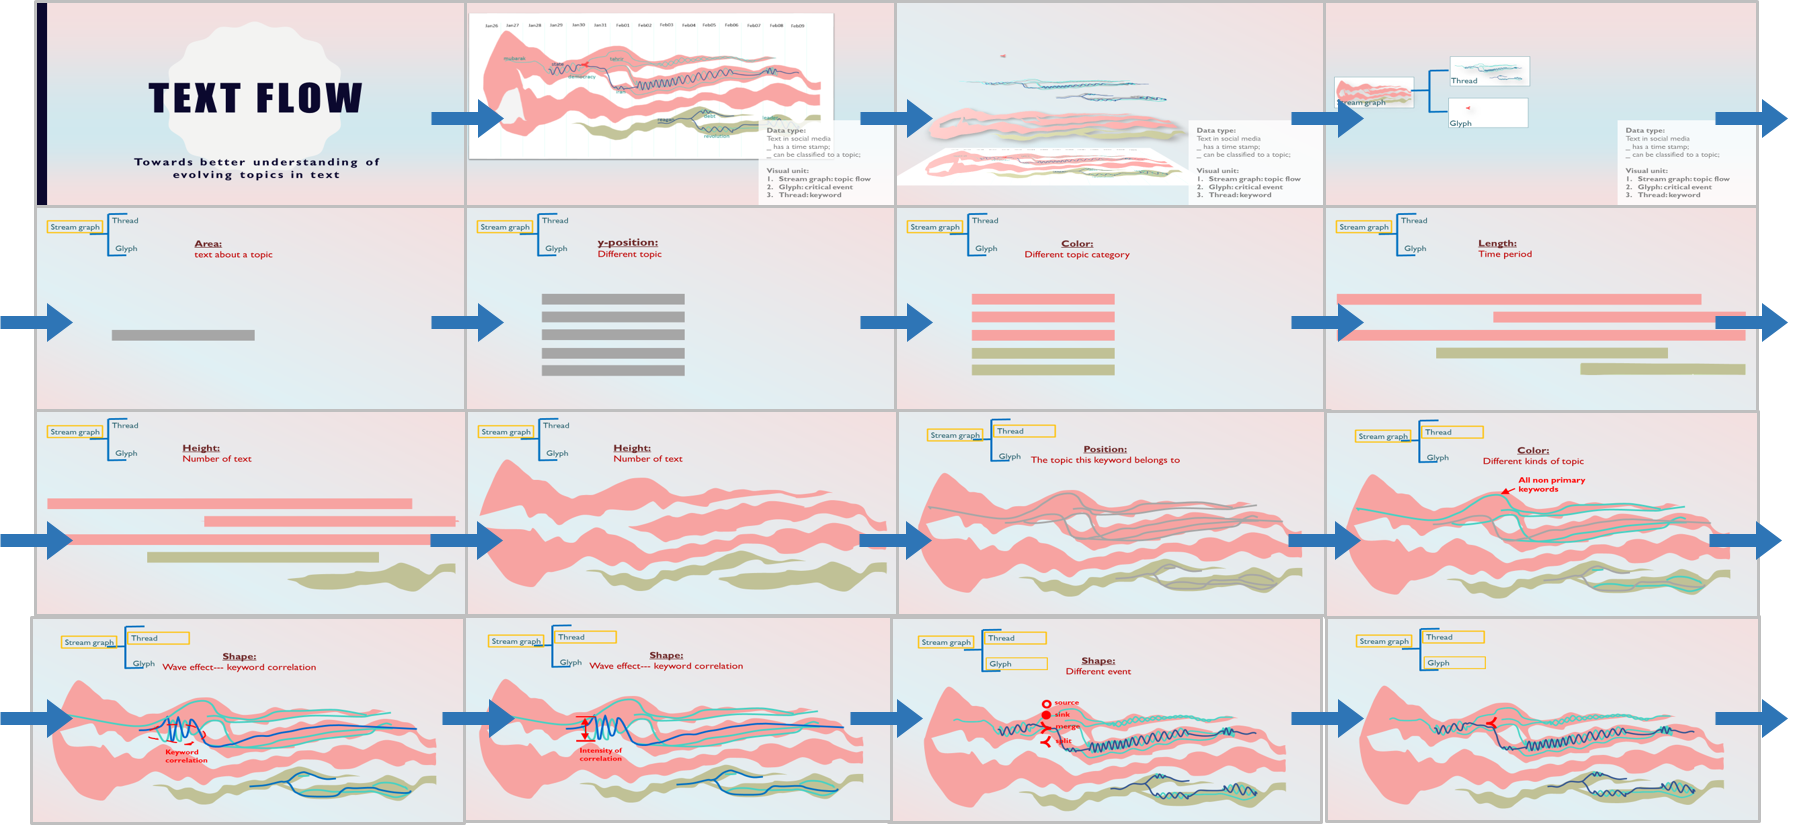
\includegraphics[width=\linewidth]{teaser}
  \caption{Example of an introduction slide show of \textit{TextFlow}\cite{cui_textflow:_2011} generated by an expert in data visualization using Narvis. This slideshow consist of (a) a cover, (b) a decomposing animation, (c) introducing the design in a constructing way.  }
	\label{fig:teaser}
}

%% Uncomment below to disable the manuscript note
%\renewcommand{\manuscriptnotetxt}{}

%% Copyright space is enabled by default as required by guidelines.
%% It is disabled by the 'review' option or via the following command:
% \nocopyrightspace

\vgtcinsertpkg

%%%%%%%%%%%%%%%%%%%%%%%%%%%%%%%%%%%%%%%%%%%%%%%%%%%%%%%%%%%%%%%%
%%%%%%%%%%%%%%%%%%%%%% START OF THE PAPER %%%%%%%%%%%%%%%%%%%%%%
%%%%%%%%%%%%%%%%%%%%%%%%%%%%%%%%%%%%%%%%%%%%%%%%%%%%%%%%%%%%%%%%%
\begin{document} 
\maketitle
\section{Introduction} %for journal use above \firstsection{..} instead
For data with complicated structure, naive data visualization like bar chart and pie chart maybe unsatisfying for a comprehensive display. By introducing metaphors borrowed from nature \cite{cao_whisper:_2012,huron_visual_2013}, applying carefully designed layout algorithms\cite{wu_opinionflow:_2014,chi_morphable_2015}, and sophisticatedly combining existing visualizations\cite{zhao_x0023;fluxflow:_2014}, novel visual presentations help people identify patterns, trends and correlations hidden in data. However, these advanced visualizations are usually not intuitively recognizable. Users need to go through some training, for example, reading a long and boring literal description, before they grasp the knowledge required to understand and freely explore a visualization.\par
What is more, even designers of these advanced visualizations suffer when they are required to introduce their design, especially when the visual encoding has complicated logic dependency, or when their audience have little prior knowledge about visualization techniques.\par
As a result, these advanced visualization technologies, in spite of
the fact that their utility has been verified by domain experts from various fields, gain little exposure outside the visual community. Main stream media is still dominated by naive visualizations, such as bar charts, pie charts and so on.

For a visualization, its core design space can be described as the orthogonal combination of two aspects: graphical elements called marks and visual channels to control their appearance\cite{munzner_visualization_2014}. But why the explanation of these two things is so complicated? 

This problem mainly arises from the fact that advanced visualization designs usually attempt to delivery a great amount of information. First, it would overload an audience if we inundated them with all the information at one time. Second, even if we tried to explain it sequentially, considering the logic dependency existing among visual elements, an improper explanation could totally confuse the audience. For example, in a node link diagram, a node should be introduced before the links connecting it. In an advanced visualization design, which has more components than just nodes and links, it is challenging to identify a proper explaning oder. Third, when digesting such a considerable amount of information, audiences can easily get distracted or forget previous information.   

Thus, to better introduce an advanced visualization, we should convey its information sequentically and in a specific order. Attention guidance and reminders are also needed to make sure that audiences are following this order, not getting distracted or forgetting previous information.

Narrative, which means “connected events presented in a sequence”, has long been used to share complex information. \cite{schmidt_living_2017}As the data visualization field is maturing, many researchers have moved their focus from analysis to presentation, making narrative data visualization an emerging topic\cite{kosara_storytelling:_2013}. Many efforts have been
made to define, classify, and provide design suggestions for narrative data visualization\cite{segel_narrative_2010,hullman_deeper_2013,gershon_what_2001}. Some visualization systems have already incorporated narrative modules into their design\cite{eccles_stories_2007,bryan_temporal_2016}. However, current work is mainly focused on communicating the conclusion of analyses, rather than guiding the audience how to read a visualization. 

Here, we present a prototype to adopt narrative techniques to create a visual encoding explanation. We
ground our work on text visualization designs, but we believe our findings and our system generalize to other types of visualization. Based on our analysis of the structure, logic dependency, and visual distraction existing in a visualization design, we develop an authoring tool to decompose a visualization, reorganize extracted visual elements, and explain their visual encodings one by one through animated transition in the form of slideshow. Through incorporating a narrative sequence, appropriate chunks of information, rather than all the information, is delivered to the audience at one time, effectively avoiding information overload. Reminders, such as questions, summarizations and repetitions are woven into the narrative sequence to enhance the audience’s memory while visual attention guidance, such as flickering, highlighting, and morphing are used to lead their attention to newly added information. (字数超了就删掉)

To the best of our knowledge, this is the first attempt to explain visual encoding with narrative. Our contributions are as below: 1). A paradigm for decomposing visualizations. It analyzes the hierarchical structure of its components, the relationships between components, and visual distraction existing. 2) A framework for explaining visualization design, which is the result of consulting theory from graphical perception process, techniques in narrative visualization, various attention cues in animation, and empirical observations of numerous visualization designs. 3) An authoring tool to generate and edit the narrative visual encoding explanation
 We conjecture our work can motivate and enable people to use more advanced visualization designs, supporting the democratization of data visualization.
 
\section {Related Work}
In this section, we review prior arts of the analysis of narrative structure in data visualization, animation in data visualization, and existing authoring tools for narrative visualizations.

\subsection{Structure of Narrative Data Visualization}
Narrative is as old as human history~\cite{cunningham_culture_2009}.  People in the fields of literature, comics~\cite{cohn_visual_2013} and cinema~\cite{schmidt_living_2017} have gone to great lengths to analyze the sequencing and forms of grouping used in a narrative, as well as how they affect the meaning a narrative tries to deliver. 

% Some people believe that work from other fields can inspire researchers in the visual data community. 
Researchers in the community of data visualization are greatly inspired by work in other fields.
Amini et al.~\cite{amini_understanding_2015} borrow concepts from comics~\cite{cohn_visual_2013} to classify and analyze the structure of data videos. Wang et al.~\cite{wang_animated_2016} adopt two representative tactics, time-remapping and foreshadowing, from cinematographers to organize a narrative sequence for visualizing temporal data. 

Some researchers, on the other side, focus on the narrative structures exclusively for data visualization. 
Satyanarayan and Heer, through interviews with professional journalists~\cite{satyanarayan_authoring_2014}, define the core abstractions of narrative data visualization as state-based scenes, visualization parameters, dynamic graphical and textual annotations, and interaction triggers. By identifying the change in data attributes, Hullman et al.~\cite{hullman_deeper_2013} propose a graph-driven approach to automatically identify effective narrative sequences for linearly presenting a set of visualizations. 

These works, however, rarely discuss the narrative structures used for explaining visual designs. We propose a narrative framework to fill this gap.

\subsection{Animation for Data Visualizations}
There is a wide discussion about the effects of animation when used in a data visualization environment.
Animation can facilitate the cognitive process. Heer and Robertson~\cite{heer_animated_2007-1} confirm the effectiveness of animation when relating data visualizations backed by a shared dataset. Ruchikachorn et al.~\cite{ruchikachorn_learning_2015}, going a step further, design morphing animations which bridge the gap between a familiar visualization and an unfamiliar one, thus introducing a new visualization design through animation. Graphdiaries~\cite{bach_graphdiaries:_2014} uses animation to help audiences track and understand changes in a dynamic visualization. 

Animation can also be an effective tool to attract and guide visual attention. Huber et al.~\cite{huber_visualizing_2005} study the perceptual properties of different kinds of animation, as well as their effects on human attention. Waldner et al.~\cite{waldner_attractive_2014} focus on a specific animation, i.e., flicker. By dividing the animation into an “orientation stage” and an “engagement stage”, they strike a good balance between the attraction effectiveness and annoyance caused by flickering. 

It is, however, noteworthy that animation, in spite of all the advantages mentioned above, can bring about negative effects when used improperly~\cite{robertson_effectiveness_2008}. In our work, we implement animations in our system guided by the results of these previous work.

\subsection{Authoring Tools for Narrative Visualizations}
The extensive needs of data communication exist not only in the data visualization field but also in journalism, media, etc. This has motivated researchers to investigate ways for authoring narrative visualization. 

User experience is of great concern when utilizing an authoring tool. Sketch story~\cite{lee_sketchstory:_2013}, with its freeform sketch interaction, provides a more engaging way to create and present narrative visualization. Dataclips~\cite{amini_authoring_2017} lowers the barrier of crafting a narrative visualization by providing a library of data clips, allowing non-experts to be involved in the production of narrative visualization. 

However, it is information delivery that is the core consideration of an authoring tool. Existing authoring tools usually choose a specific type of narrative visualization based on the information type~\cite{amini_authoring_2017, fulda_timelinecurator:_2016}. Meanwhile, integrating an authoring tool for narrative visualization with a  data analysis tool has become a trend since it effectively bridges the gap between data analysis and data communication~\cite{eccles_stories_2007, bryan_temporal_2016,lee_more_2015}. 
 
These tools offer inspiring user interaction design as well as good examples to implement narrative visualization. However, they treat visual encodings as cognitively obvious attributes that can be universally recognized without a formal introduction, which is not appropriate for introducing visual designs. In our paper, we propose an authoring tool specified for presenting visual designs in a narrative way. 
% making them inapplicable in our case. 

\subsection{Decomposition of Data Visualization}
Clarifying the design space of a data visualization can help people get a better understanding of how it is constructed. Munzner~\cite{munzner_visualization_2014} proposes that it ``can be described as an orthogonal combination of two aspects: graphical elements called marks and visual channels to control their appearance''. Borrowing the concept of physical building blocks such as Lego, Huron et al.~\cite{huron_constructive_2014} extends the design space of a data visualization, defining the components of a data visualization as a token, token grammar, environment and assembly model.

Such theoretical work motivates the designers of visualization tools to contribute efficient high-level visualization systems rather than low-level graphical systems~\cite{bostock_protovis:_2009,mendez_ivolver:_2016}. 

On the other hand, theoretically identifying the basic components of a data visualization enables people to physically extract them, and remap them to an alternative design without involving any programming work. Harper and Agrawala~\cite{harper_deconstructing_2014} contribute a tool that extracts visual variables from existing online visualization designs to generate a new design. Huang et al.~\cite{Huang:2007:SUI:1284420.1284427} propose a system that recognizes and interprets imaged
infographics from a scanned document. Revision~\cite{savva_revision:_2011} applies computer vision methods to recognize the types, marks, encodings of a data visualization, and allows the users to create a new design based on these data. 

However, these decomposing methods exclusively focus on simple visualization designs, such as bar chart, line chart, dot chart, and are not applicable for complex visualization designs, which assemble miscellaneous visualization approaches to realize a novel presentation. Moreover, these methods are not specified of explaining a visual design, thus giving no consideration for graphical perception process and visual attention shift. In this work, we attempt to propose a model which can fill this gap.


\section{Introducing a data visualization} \label{analysis}
To help people better understand a data visualization design, we propose a method that introduces a data visualization through constructing, which has been proven as an effective teaching method\cite{huron_constructive_2014, chapman_constructive_1988} . Thus, there are three questions we need to answer: ``\textit{what are the basic components that compose a data visualization? }'' ,``\textit{what is the relationship between these components? }'', ``\textit{How should we deal with these relationships in our narrative?}''. At the same time, considering the large number of graphical elements employed in a data visualization design, we should eliminate the visual distraction to keep audience's focus on the target.

\subsection{Compositions of a Visualization}\label{compositions}
We propose a model that decomposes a visualization into three levels of structure: visual primitives, visual units, and then an advanced visualization design. 
We apply this hierarchical structure theory to ``Opinionseer''~\cite{wu_opinionseer:_2010} and decompose it, as shown in Figure~\ref{fig:hierarchic}. 

\noindent
\textbf{A visual primitive} is one graphic element whose visual channels, such as color, width, height, are mapped to data attributes with certain visual grammar.  For instance, a point whose size and color are encoded is a visual primitive. Size is a visual channel, and``size indicates the importance score'' is a visual grammar. 

\noindent
\textbf{A visual unit} is the assembly of visual primitives based on a certain construction rule, as Table~\ref{tab:unit} show. 
%For the taxonomy of constructing rule, we refer the ``alignment method'' in \cite{kucher2015text} but make it more specific. 
A visual primitive can assemble different visual units by following different constructing rule. For example, the visual primitive, dot, can assemble scatter plot, spiral dot chart, or circle packing chart by following radial, orthogonal, or metric-based construction rule, respectively. We are not pretending that our table includes all existing visual units, since new design is proposed constantly. A visual unit is the smallest functional unit of a visualization. Note that we only consider statical visualization. People might employ two visual primitives in an animated visualization unit. For example, Huron et al.\cite{huron_visual_2013} employed two visual primitives to mimic the physical process of sedimentation for visualizing data streams. 

\noindent
\textbf{A visualization} can be treated as the combination of visual units. A naive visualization can be as simple as one visual unit while an advanced one is usually the combination of several units. 
%It doesn't simply put all visual units together but constructs them based on their relationships, as described in Section 3.2.1.
% with certain connections \siwei{what is certain connections? can you give an example?} with each other, which is detailedly discussed in section 3.1.2.\siwei{where is section 3.1.2?}

\begin{figure}
 \centering % avoid the use of \begin{center}...\end{center} and use \centering instead (more compact)
 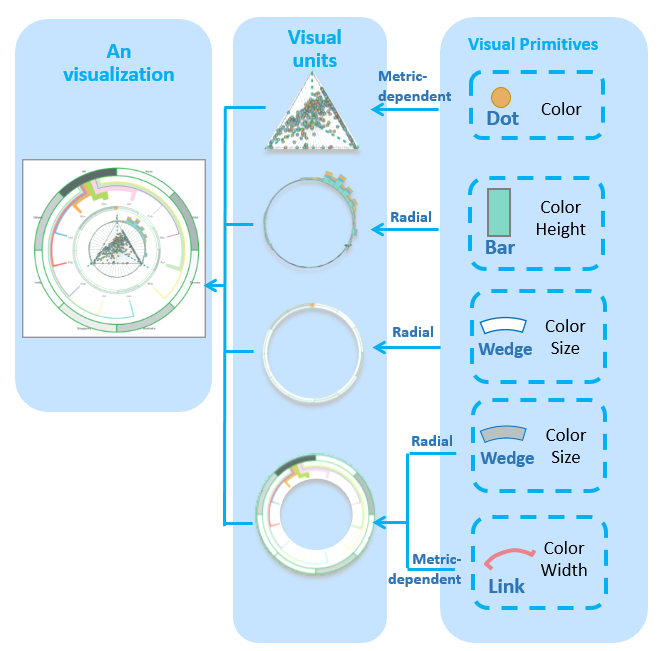
\includegraphics[width=\columnwidth]{hierarchic}
 \caption{An example of the hierarchical structure of a visualization, Opinion Seer\cite{wu_opinionseer:_2010}}
 \label{fig:hierarchic}
\end{figure}

%\begin{figure}
%\begin{minipage}{\columnwidth}
% \centering % avoid the use of \begin{center}...\end{center} and use \centering instead (more compact)
% 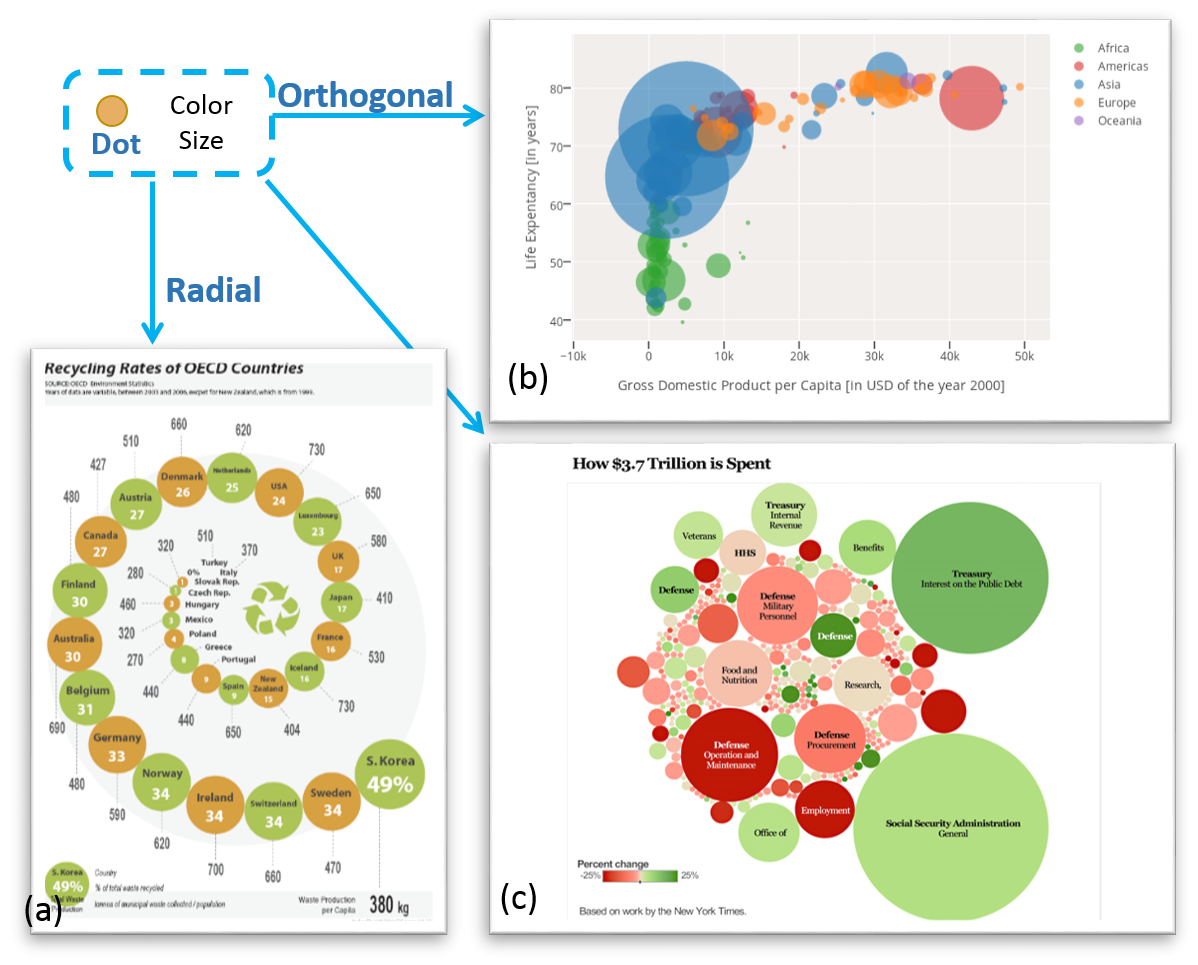
\includegraphics[width=\columnwidth]{assemble}
%\caption[assemble]
%{
%A dot, whose color and size are encoded, can assemble 
%(a) a dot spiral chart
%\protect\footnotemark{}
%    , (b)a dot packing chart
%  \footnotemark{}
%  , and (c)a bubble chart
%  \footnotemark{}
%   by following different construction rules.
%}
%\end{minipage}
%\label{fig:hierarchic}
%\end{figure}
%\footnotetext{https://www.pinterest.com/pin/16536723602037537/}
%\footnotetext{https://plot.ly/~etpinard/84.embed}
%\footnotetext{https://bl.ocks.org/mbostock/4063269}

%\begin{table*}[tb]
%  \caption{A taxonomy of visual units.\notsure{How to avoid the name ambiguities}}
%  \label{tab:unit}
%  \small
%  \centering
%  \begin{tabular}{|p{1.2cm}|p{1.2cm}|p{1.2cm}|p{1.2cm}|p{1.2cm}|p{1.2cm}|p{1.2cm}|p{1.2cm}|p{1.2cm}|}
%  \toprule
%   \textbf{} &\multicolumn{2}{|c|}{Polar Coordinates} &\multicolumn{3}{|c|}{Orthogonal Coordinates}&\multicolumn{3}{|c|}{Metric Dependent}   \\ 
%  \midrule
%  
% \textbf{} &\textbf{Radial} &\textbf{Spiral} &\textbf{Orthogonal} & \textbf{Parallel Align}&\textbf{Map}&\textbf{Cluster}&\textbf{Force-direct}&\textbf{Others}   \\ 
%  \midrule
%  \textbf{Dot} &    &Spiral Dot Chart&Scatter Plot, Bubble Chart & Dot Plot & Bubble Map &  Circle packing    &TopicPanorama\cite{7042494}  &    \\
%  \midrule
%  \textbf{Line}&  Radar Chart   &  Spiral Plot    &Node-link Diagram, Line Chart & Parallel Coordinates, Arc Diagram &    &   &     & \\ 
%  \midrule
%   \textbf{Flow}&  Chord Diagram   &    & &Parallel Sets, Sankey Diagram & 
%   Flow Map  &   &   &\\
%  \midrule
%  \textbf{Area}&    &Area Spiral Chart &Stream Graph &  & & &   &\\ 
%  \midrule
%  \textbf{Bar}&      Radial Bar Chart & Spiral Bar Chart  & Candlestick Chart & Bar Chart  &    &    &    &\\
%  \midrule
%  \textbf{Cell}& Sunburst Diagram  &    & Matrix, Tree Map &     & & &   &\\
%  \midrule
%  \textbf{Wedge}& Pie Chart, Donut Chart &  &   &   &  &    &   &\\
%  \midrule
%  \textbf{Text}&    &Parallel Tag Cloud \cite{collins2009parallel} &    &  Sentence Tree  &     &Word Cloud  &   &    \\
%  %\midrule
% % \textbf{Image}& & &Heatmap Matrix &Heatmap &\\
%  \bottomrule
%  
%  \end{tabular}
%  \vspace{1mm}
%\end{table*}

\begin{table}[tb]
  \caption{A taxonomy of visual units.\notsure{How to avoid the name ambiguities}}
  \label{tab:unit}
  \small
  \centering
  \begin{tabular}{p{1.2cm}|p{1.6cm}|p{1.6cm}|p{1.6cm}}
  \toprule
  \textbf{} &\multicolumn{2}{|c|}{\textbf{Absolute Position}} &\textbf{Relative Position}   \\ 
  \midrule
 \textbf{} &\textbf{Radial} &\textbf{Orthogonal, Align, Map} &\textbf{Metric-based}   \\ 
  \midrule
  \textbf{Dot} &Spiral&Dot Chart, Scatter Plot, Bubble Chart, Bubble Map &Circle packing, TopicPanorama\cite{7042494}\\
  \midrule
  \textbf{Line}&  Radar Chart, Spiral Plot    &Line Chart, Parallel Coordinates, Arc Diagram &  Force-directed Node-link graph   \\ 
  \midrule
   \textbf{Flow}&  Chord Diagram   &Parallel Sets, Sankey Diagram, 
   Flow Map  & \\
  \midrule
  \textbf{Area}&  Area Spiral Chart &Stream Graph &  \\ 
  \midrule
  \textbf{Bar}&      Radial Bar Chart,Spiral Bar Chart  & Candlestick Chart, Bar Chart  &   \\
  \midrule
  \textbf{Cell}& Sunburst Diagram  &Matrix, Tree Map &  \\
  \midrule
  \textbf{Wedge}& Pie Chart, Donut Chart &  &  \\
  \midrule
  \textbf{Text}&    &  Sentence Tree  & Word Cloud \\
  %\midrule
 % \textbf{Image}& & &Heatmap Matrix &Heatmap &\\
  \bottomrule
  
  \end{tabular}
  \vspace{1mm}
\end{table}

\subsection{Relationships Between Compositions}
We first describe the relationship between conceptual compositions, then offer suggestion for narrative sequence based on these relationships. Notice that we skip the relationship between viusal primitives since there is only one kind of visual primitive in a visual unit. 
\subsubsection{Relationships Between Visual Units}
A visualization can be specified as the combination of several visual units. 
% Through observing the approaches people apply to design new visualizations, 
By observing how visualizations are designed,
we define four types of relationship between visual units: irrelevance, relevance, enhancement, and dependency. 

\textbf{Irrelevance} is a bi-directional relation meaning two visual units are independent and do not share any visual channel.
For example, 2 donut charts, Figure~\ref{fig:relationship}(a) and Figure~\ref{fig:relationship}(b), are applied to illustrate the distribution of age and gender groups respectively in a population. They are put together in Figure~\ref{fig:relationship}(c) just for space-efficiency and there is no correlation between these two charts. 

\noindent
\textbf{Relevance} refers to that two visual units share some visual grammar and it is a bi-directional relation. 
For example, a line chart, Figure~\ref{fig:relationship}(d), indicates the temperature over a time period, and a bar chart, Figure~\ref{fig:relationship}(d), indicates the precipitation over a time period. They are put together in Figure~\ref{fig:relationship}(e) and they share the same visual grammar of horizontal position.  
%\siwei{what is the difference between visual grammar and visual channel? why horizontal position is visual grammar rather than visual channel?}
%\notsure{According to our survey, color and position are the most commonly shared visual encodings, which might be the result that color and position usually encoded with simple while crucial information. }


\noindent
\textbf{Enhancement} is an one-way relationship. If one visual unit ``A'' is the enhancement of another visual unit ``B'', it means that ``A'' is imported into ``B'', replaces some graphical elements of ``B'', thus enables the representation of some data attributes that ``B'' alone fails to convey. Suppose there are 5 types of area in a park. A bar chart, Figure~\ref{fig:relationship}(h), illustrates their average price per unit area, a chord diagram, Figure~\ref{fig:relationship}(g), illustrates how passengers travel through each area. In Figure~\ref{fig:relationship}(i), the bar chart take the place of node segments, which has the same height, in a chord diagram, resulting in a novel and informative visualization.
 
Enhancement widely exist in the advanced visualization design, such as the heat map mapped upon the steams in a theme river~\cite{wu_opinionflow:_2014}  and usage of glyphs to enhance the meaning of nodes in a multidimensional scaling plot~\cite{chen_peakvizor:_2016}. 

\noindent
\textbf{Dependence} is a one-way relationship. If one visual unit ``A'' is dependent on ``B'', it means that ``A'' reveal some information that results from the visualization of ``B''. For example, a multiple dimensional scaling (MSD) map, Figure~\ref{fig:relationship}(j), shows the similarity between each restaurants in a city. A contour map, Figure~\ref{fig:relationship}(h), is then added to the MSD map to \notsure{show the most common type of restaurants, which information can hardly be obtained from the dataset but quite evident from the MSD map}, as in Figure~\ref{fig:relationship}(i).The biggest difference between "\textbf{enhancement}" and "\textbf{dependence}" is that 1)\textbf{enhancement} still illustrate the data attributes in the dataset, while \textbf{dependency} reveals the new knowledge we obtain from adopting a previous visualization to the dataset; 2)\textbf{enhancement} replace original graphical elements of other visual design while \textbf{dependence} add new graphical elements.

A proper narrative sequence of visual units should take the relationships between them into consideration. For irrelevance, it doesn't matter whether these two visual units are explained sequentially. For relevance, these two visual units should be explained one after another. Since relevance is bidirectional, it doesn't matter which one is explained first. For dependency and enhancement, which are unidirectional, the two visual units should be explained sequentially in a specific order. 
 Thus, we display the correlations between units in a tree diagram where a child node is the enhancement/dependence of its parent node and sibling nodes have relevance. A proper narrative sequence can be obtained by running a deep first search on this tree diagram. 

%\subsubsection{Relationships Between Visual Primitives}
%%\siwei{There are some notes: 1. do not mention usually has 1 or 2 primitives. it is flawed. 2. Candlestick chart and error bar are quite similar expect their context. why one has no dependency and the other has logical dependency? 3. do not use two ``such as'' in one sentence.}
%%The inner relationship between visual primitives is relatively simple.
%%A visual unit usually has 1 or 2 visual primitives. 
%%
%%\notsure{
%The relationship between two visual primitives of one visual unit are usually self-evident. One primitive either has no dependency on the other one, such as the bar and line in \textit{Candlestick Chart}, or has high and evident dependency.  This dependency can be logical, such as the line and bar in \textit{error bar chart}, or spacial, such as the node segment and arc in \textit{chord diagram}, or temporal, such as the stream and dot in \cite{liu_online_2016}


\begin{figure}[tb]
 \centering % avoid the use of \begin{center}...\end{center} and use \centering instead (more compact)
 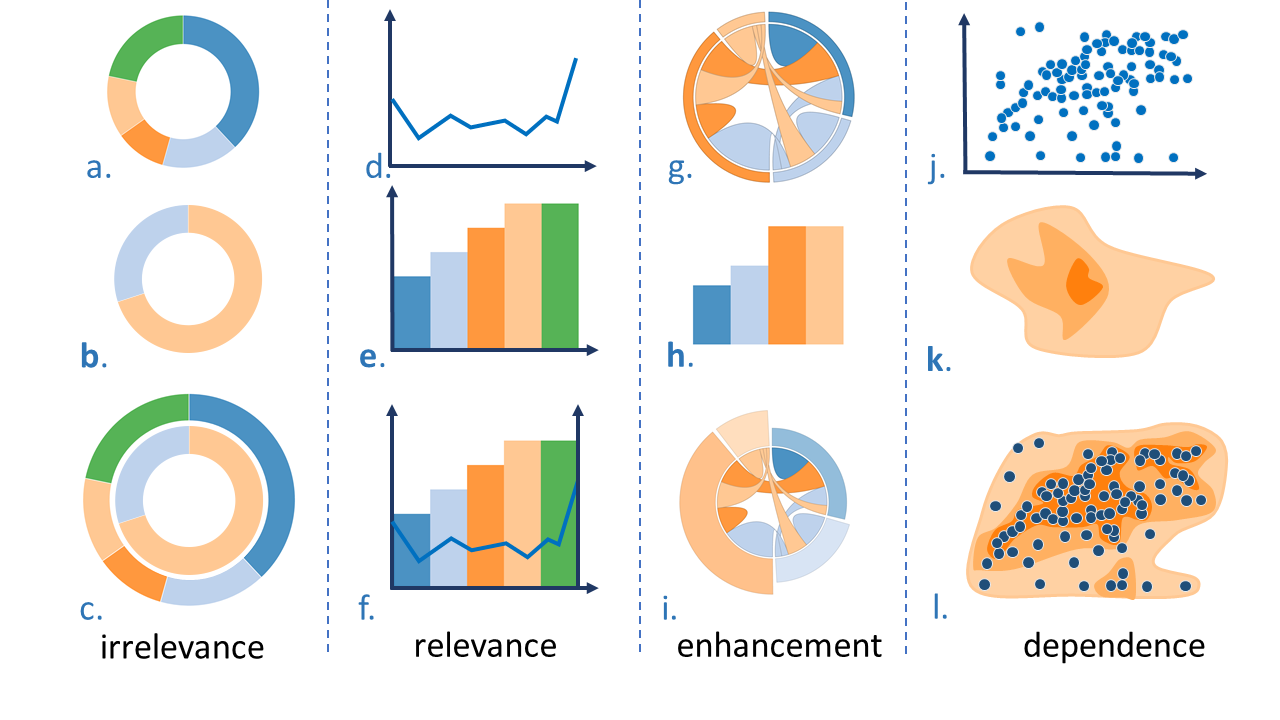
\includegraphics[width=\columnwidth]{unit_relationship}
 \caption{Illustration of the 4 types of relationship between visual units}
 \label{fig:relationship}
\end{figure}

\subsubsection{Relationships Between Visual Channels}
For a visual primitive, different channels are encoded with different data attribute. Thus, they are usually separated and have no logic dependency upon others. It's hard to determine a narrative sequence from their inner logical dependency. 

Therefore, we define two metrics to order the explaining of visual channels: \textbf{the complexity of their encoded information} and \textbf{saliency of their visual appearance}.

First, the order of decreasing visual saliency can facilitate graphical perception~\cite{cleveland_graphical_1984}. Even though different channels have intrinsically different perceptual salience and channel with high salience will suppress the expression of other, such salience strength can be influenced in a task-dependent manner ~\cite{nothdurft_salience_2000}. By introducing the channel with high saliency first, we remove it from the task list in our mind~\cite{itti2001computational}, decrease its saliency and give other channels more chance to attract the limited human attention. 

Second, the order of increasing complexity leads to an effective learning process. “Easy to difficult” practice has been long used and confirmed to be effective for learning new tasks~\cite{bliss_effects_1992}.
 
The visual saliency of different channels is relatively constant and  well defined ~\cite{munzner_visualization_2014,cleveland_graphical_1984}, while their information complexity varies in different designs. Thus, an effective narrative sequence is a trade-off between these two metrics. 

%\subsubsection{Non-linear Sequence}
%So far, all the narrative explanation we discussed is linear. However, reading a lengthy, extremely detailed instruction maybe tedious. A good narrative explanation should include non-linear design, allowing users to skip uninterested parts, go back to previous information and freely switch between different parts. Also, users should be allowed the flexibility to choose explanations at different levels of details. 

\subsection{Attention Orientation}
To keep audience focus on the target object, it is necessary to identify visual distractions so that measurements can be taken to avoid them. 
We identify two kinds of visual distractions: the one from context and the one from sibling channels, which refer to the visual channels belonging to the same visual primitives. 

\subsubsection{Visual distraction from the context}
This kind of distraction has been widely discussed in the field of object detection and human visual attention ~\cite{nothdurft_salience_2000, standage_modelling_2005}. Its intensity is mainly  determined by spatial distance and appearance similarity ~\cite{wolfe_guided_1994}. 
Focus + Context, which might be the most popular techniques for this problem, make uneven use of graphic resources to discriminate focus from their context. At the same time, adding dynamic changes to focus elements has also been demonstrated as effective under various conditions\cite{waldner_attractive_2014}. We support easy implementation of these techniques in our system. 

\subsubsection{Visual distraction from sibling channels}
A visual primitive usually has more than one visual channels. Thus, when recognizing one primitive, the channels with high visual saliency can significantly influence the expression of other channels. For example, color can be a strong noise when focus is supposed to be the shape. By applying animated transition and revealing only one channel at a time, as demonstrated in \notsure{Fig1, the second line}, we are able to reduce such distraction.



\section{Design Considerations}
In this section, we first describe our understanding of two groups of end users, i.e., editors and general audience. Then, we distill design tasks to guide our design and development of Narvis.

\subsection{User Perspectives and Methods}

Narvis aims to offer an efficient, expressive and friendly authoring tool for experts in data visualization, assisting them to create a slideshow to introduce advanced visual design to general audience.  
Hence, we identify two different user perspectives: the editors and the general audience perspectives. Editors are visualization experts who have the need to create a slideshow to present visual designs. General audience have no prerequisite for visualization. They gain understanding of a visual design through the slideshow created by the editor. 

To understand the current practice of making slideshows and the experience of reading tutorials, we collaborated with two teaching assistants (TAs) of a Data Visualization course and seven undergraduate students (UGs) taking this course. The two TAs are postgraduate students whose research interests are information visualization. Their duty of this course involves making slides to introduce visual designs from major publications in the field of visualization. The slides should cover fine-grained description to help students review them after class. The seven UGs have no prior experience in visualization, and have taken this course for no more than one month.  

We began by conducting semi-structured interviews with TAs, whom we identified as editors, and UGs, as general audience. During the interviews with TAs, we asked their workflows of making slideshows and explaining visual design. To identify opportunities for Narvis, we also asked them to enumerate a list of challenges faced in the workflows. The interviews with UGs are semi-structured as well. We asked their comments in reading the slideshows and attending course lectures. Then, we used mind-mapping to find clusters in their comments that defined goals for an ideal slideshow. 


\subsection{Design Tasks}
Based on our observations and the interviews, we categorize six design tasks to guide the design of Narvis. Three tasks, denoted as DE, are originated from the interview with editors, i.e., the two TAs, and other three tasks (DA) are from general audience (UGs).

%Our premise is that the editor is familiar with a visualization design but unclear how to educate his audiences in an efficient way. Since the background of the audiences cannot be guaranteed, we assume they all have no prior knowledge in data visualization. 
\noindent
\textbf{DE1. Emphasis on  efficiency.}
TAs used presentation tools, such as Power Point\footnote{https://office.live.com/start/PowerPoint.aspx}and KeyNote\footnote{http://www.apple.com/keynote/} to introduce visual designs. However, these tools are for general purpose and not tailored for visualization presentation. 
For example, "focus + context" techniques are widely used in data visualization to guide the user’s attention to the region of interest \cite{doleisch2003interactive, kosara2002focus+}. It requires exaggeration or suppression of the visual channels, like hue, luminance , sharpness, or size, of graphical elements, which are hard to perform in these common presentation tool. 
% Moreover, with the large number of visual encodings existing, she fails to determine an optimized order for explaining them. Even though she has many years of experience in data visualization, she never think about this issue before. 
%Splitting a visualization into fine-grained graphical elements and combining them into logic flow are tedious and time-consuming with existing tools. 
%Therefore, automatic decomposition of visualization and composition of graphical elements are necessary for facilitating design and production of a slideshow.
% TAs require an efficient approach to generate a slideshow introducing visual design.

\noindent
\textbf{DE2. Suggest options.}
People with extensive experience in designing data visualization can have little knowledge about how to present a visual design. 
Thus, suggesting design options to them for creating a comprehensive slideshow is demanding. Many presentation tools already offer this kind of service. For example, Power Point Designer\footnote{https://support.office.com/en-us/article/About-PowerPoint-Designer-53c77d7b-dc40-45c2-b684-81415eac0617} automatically generate a list of professionally designed layouts based on the contents. However, these suggestions focus on general issues, especially on aesthetics, and give no special consideration for presenting a visual design.
For example, composing a clear narrative sequence from all the visual grammar employed can facilitate the perception process. A list of design options can help editors quickly ideate on how to organize the narrative sequence and convey the insights of a visual design. However, no available presentation tool supports such service. 
%\siwei{your logic is: other tools have no special consideration for doing sth. Reviewers may think: why they should have such consideration? You should emphasize these consideration is important in visualization because of some reason.}
%The complicated relationship, spatial and logical alike,  between different graphic elements is one of the biggest barriers that hinders the effective presentation of a visual design. Howe like Power Point Designer"
%By encouraging users to refine the clusters of graphic elements, to figure out relationship between visual units by editing a unit tree, and to modify the narrative templates we offered, we aim at motivating users to sort out the structure of a visualization, which will then result in a better-organized narrative sequence. 

\noindent
\textbf{DE3. Collect feedback.} \textit{``When students read my slides, I do not know whether they can follow the logic, or whether the slides cover enough details for them to grasp the visual design.''}, one TA commented. 
% When giving a lecture, TAs are able to understand how their slides and logic are accepted through in-class interactions. 
Collecting feedbacks of audience is crucial for editors to revise their slideshow, making it more understandable and attractive.  

%We implement a click collector which will automatically record click activity when audience view the explanation in our system. The click stream data can reveal information about viewing order, for example, the audience might skip one slide or go back to revisit another, the time spent on each slide, the degree of understanding at each part.The audience can also write down their comments while reviewing such an introduction slide show. Editor can adjust the narrative sequence as well the level of details based on these feedbacks. 
\noindent
\textbf{DA4. Avoid information overload.} 
All UGs complained that they had experienced information overload in reading slides. 
%Though they might separate an informative slideshow into parts and read one part at a time, they might miss some when the information in one slide is overwhelming.
% We distinguish the amount of information in the slideshow and in one slide. Audience  However, 
When the information in one slide is overwhelming, it is common for they to miss important visual encodings. 
The slideshow should be well designed to ensure that the amount of new information in each slide is appropriate. 

\noindent
\textbf{DA5. Avoid unconscious ignorance.}
Experts in data visualization, i.e. the TAs of the course, prone to treat some visual grammars as self-evident that need no  explanation. However, the lack of information confuses the UGs, who have no prior knowledge of visualization. 
Considering the importance of information integrity to a comprehensive slideshow, we need a mechanism to guarantee that all visual grammars are explained. 

\noindent
\textbf{DA6. Keep the sense of overview}
Grouping slides into sections, and inserting visual notice, like a progress bar, to indicate the overall structure is an effective and widely used presentation skill \siwei{if you say they are widely used, please cite}. 
However, partly due to the lack of a clear narrative structure, this technique is rarely used in the presentation of a visualization, in spite of the demands from audiences.

 \siwei{do not say the technique is rarely used in visualization because it is not convincing. say how the technique can help visualization presentation, therefore it is important.}



\section{Narvis: System Design and Implementation}

% Thus, it has two kinds of users: editors, the data visualization experts who use Narvis to create an explanation slideshow, and audiences, the general audience who watch the slideshow created by ediors.

Guided by the theory model discussed in Section~\ref{analysis},  we design and implement Narvis, an authoring tool for crafting slideshows for the presentation of visualization. The workflow of Narvis consists of three phases (Figure ~\ref{fig:overview}), i.e., Automatic Analysis Phase, Authoring Phase, and Viewing Phase.

% The workflow of Narvis includes three phases (Figure \siwei{ref}):  In Automatic Analysis Phase, the system accepts the input visualization, extracts graphical elements and classifies them into groups for further edit. 
% In Human Editing Phase, editors will be involved to modify the output from the Automatic Analysis Phase, and use the templates Narvis provide to craft a explanation slideshow. 
% In Reviewing Phase, audience can assess the slide show generated in Human Editing Phase. Their click activity and comments will be recorded and send to the editors, helping them improve the quality of the slide show. 

\begin{figure}
 \centering % avoid the use of \begin{center}...\end{center} and use \centering instead (more compact)
 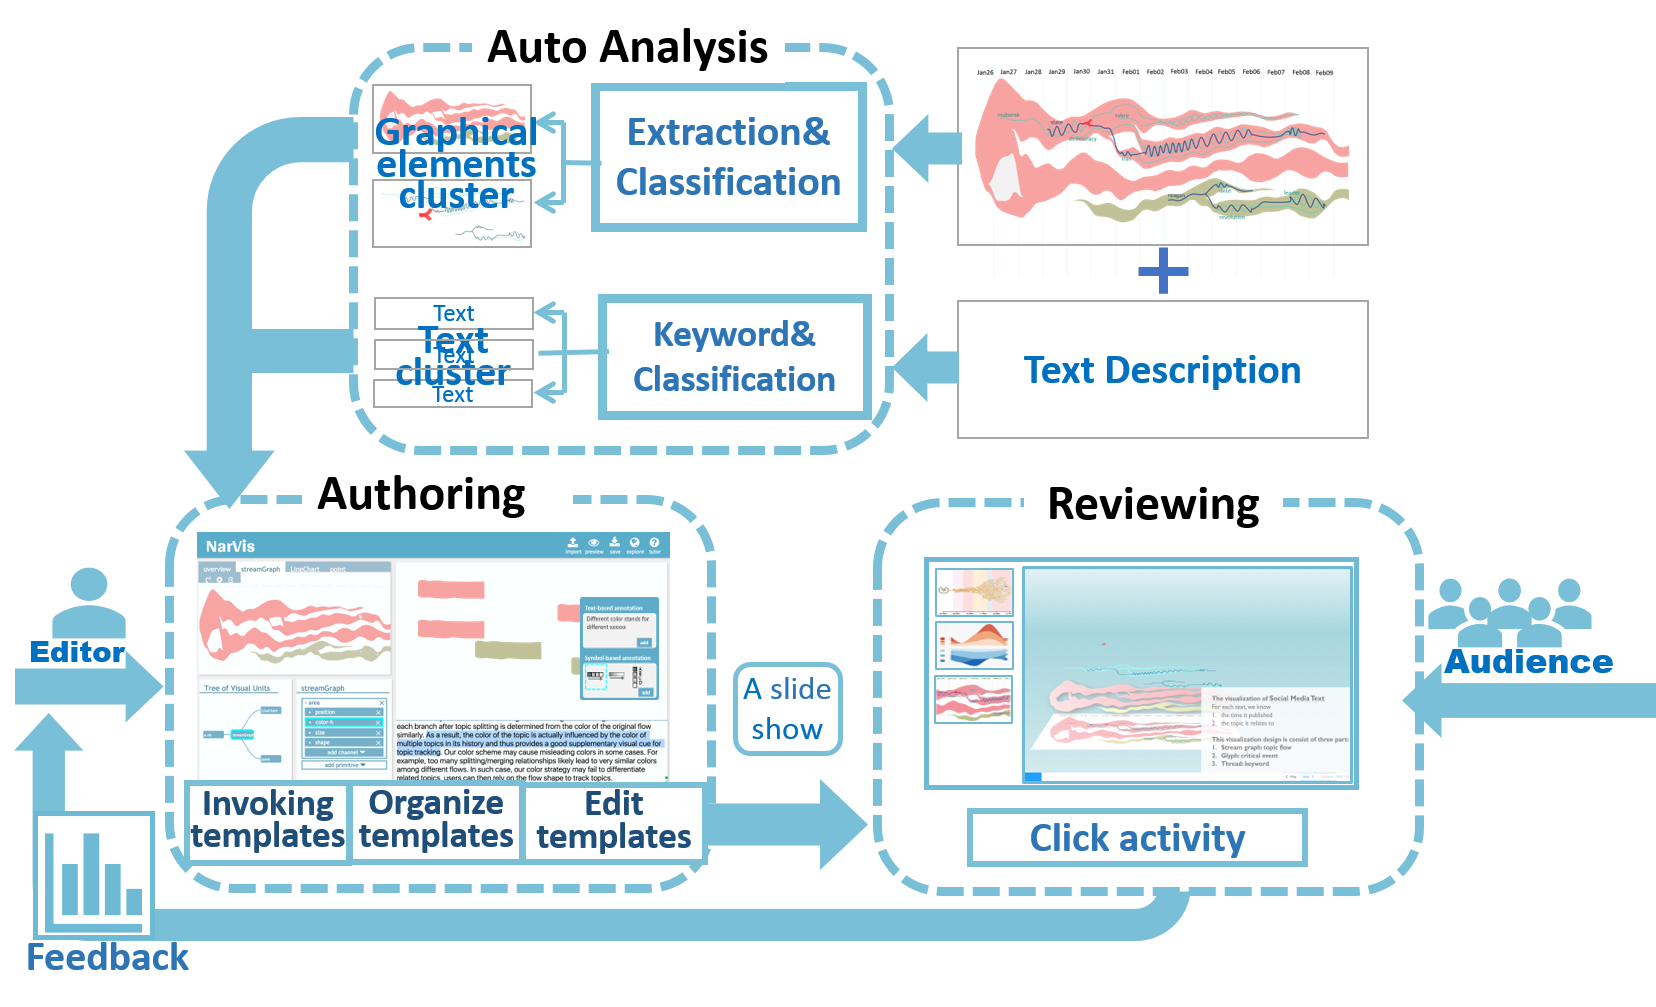
\includegraphics[width=\columnwidth]{overview}
 \caption{The system overview}
 \label{fig:overview}
\end{figure}

\subsection{Phase1: Auto Analysis}

% The auto analysis has two parts: one for input image and one for input text. It automatically extract the graphic elements and divide them into different cluster, facilitating later editing.(DE1) Note that the textual input is not necessary but it provides hints when editors add annotations manually in the Human Editing Phase.(DE1)

The input of Narvis includes two parts: one image presenting a visual design (mandatory) and a piece of text describing the design (optional). Considering that the vast majority of visualizations are only available as bitmap images, we offer an algorithm to detect and extract the graphical elements from the input image. Here, we explain the basic idea of how Narvis analyzes these input sources to facilitate further authoring. 
\begin{algorithm} 
        \caption{Object Detection}  
        \label{alg:alg1}
        \begin{algorithmic} % line number
            \Require A bitmap in the form of a two-dimensional array: $A$
            \Ensure A list of objects: $B$
            \State $B \gets \{\}$
            \ForAll{$pixel (x,y) \in A$} 
                \If{no mark on $pixel(x,y)$}
                    \State $Q \gets \{(x,y)\} $
                    \State $Obj \gets \{\}$
                    \ForAll{$(x,y) \in Q$}
                        \State $Q = Q - \{(x,y)\}$
                        \State $Obj = Obj \cup \{(x,y)\}$
                        \ForAll {$(x',y')$ which $|x'-x|+|y'-y|\leq2$ and no mark on $pixel(x',y')$}
                            \If{$pixel(x,y)$ and $pixel(x',y')$ have similar color}
                                \State $Q = Q \cup \{(x',y')\}$
                                \State Make a mark on $(x',y')$
                            \EndIf
                        \EndFor
                    \EndFor
                    \State $B = B \cup \{Obj\}$
                \EndIf
            \EndFor
            \State \Return{$B$}
        \end{algorithmic}  
    \end{algorithm} 
    
    
    \begin{algorithm}  
        \caption{Object Clustering} 
        \label{alg:alg2} 
        \begin{algorithmic} % line number
            \Require A list of objects: $A$, the number of clusters: $N$
            \Ensure A list of objects: $B$
            \State $E \gets \{\}$
            \ForAll{$a_1 \in A$}
                \ForAll{$a_2 \in A$ and $distance(a_1,a_2) \leq L$} \Comment{$L$ is a parameter that accelerates our calculations}
                    \If{$a_1$ and $a_2$ have similar color}
                        \State $d \gets$ the distance between $a_1$ and $a_2$
                        \State $E \gets E \cup \{(a_1, a_2, d)\}$
                    \EndIf
                \EndFor
            \EndFor
            \State $B \gets A$
            \State $E \gets$ sort $E$ by the $d$ of each elements in descending order
            \ForAll{$(a_1,a_2, d) \in E$}
                \State $b_1 \gets b|b\in B, a_1 \subseteq b$
                \State $b_2 \gets b|b\in B, a_2 \subseteq b$
                \If{$b_1 \neq b_2$}
                    \State $B = (B - \{b1\} - \{b2\})\cup \{b1 \cup b2\}$
                \EndIf
                \If{$|B|\leq N$}
                    \State break
                \EndIf
            \EndFor
            \State \Return{$B$}
        \end{algorithmic}  
    \end{algorithm} 
    
\subsubsection{Analysis of Input Image}
% The auto analysis of input image has three main steps. It first detects all primitives that it finds in the given image and also detects any labels that are present in the visualization. It will then cluster objects that are spacially linked and extract non-target objects. Finally, it will fill in any empty spaces left inside objects from extraction with the appropriate color so as to show the target object in its entirety.
The analysis of the input image includes two steps, object detection and object clustering.
% and object recovery.

% The first step, object detection, is done by iterating through all the pixels on the bitmap. 
\noindent
\textbf{Object detection.} We iterates through all pixels, and clusters all the pixels that are i) neighbors and ii) have the similar color through a modified Breath-first search algorithm (see in Algorithm~\ref{alg:alg1}). Simple objects, such as a bar in a bar chart, a node in a scatter plot, are detected and extracted after this step.

\noindent
\textbf{Object clustering.} All the objects with spatial and appearance similarity are clustered to allow an efficient manipulation, as described in Algorithm~\ref{alg:alg2}. For example, all the nodes in a scatter plot should be put in one cluster, instead of letting the editor add them one by one manually.     
%\noindent 
%\textbf{Object recovery.} Once we have completed extraction, we have the issue of these white spaces. The reason this is an issue is because an extracted object might have been dividing two objects, and so when it is extracted, we lose the boundary between our target object and another object, which can cause confusion as to whether that white space should be colored in or not. To solve this boundary problem, we create a queue of the white spaces, with each data point giving the starting and ending point of that space. We then look at the intervals between enclosed white spaced objects, if that interval is above a threshhold, we take that white space to not be part of our object. If it is below our threshhold, then we enclose the white space with the target objects color, creating a boundary for it. The main difference is that for objects not within our target object, we do not create a boundary, whereas objects within our target object are enclosed with the target objects color.

\subsubsection{Analysis of Input Textual Description}
For the input textual description, we offer a keyword detection and classification algorithm, which is based on a dictionary of terms that are identified as highly related with visual grammars. e.g. the word ``length'' and ``encodes'' ,are highly correlated with the  visual grammar of size. We extract all the sentences containing the terms in our dictionary, and cluster them based on the terms they have.

The algorithm we proposed is a compromise between efficiency and performance. It is a heuristic algorithm for images with high quality and clear edges, but its performance can be improved by adopting other well-established algorithm, such as an algorithm based on patch detection and clustering \cite{savva_revision:_2011} and an algorithm based on edge maps \cite{huang2003model}.


    
    
\begin{figure}
 \centering % avoid the use of \begin{center}...\end{center} and use \centering instead (more compact)
 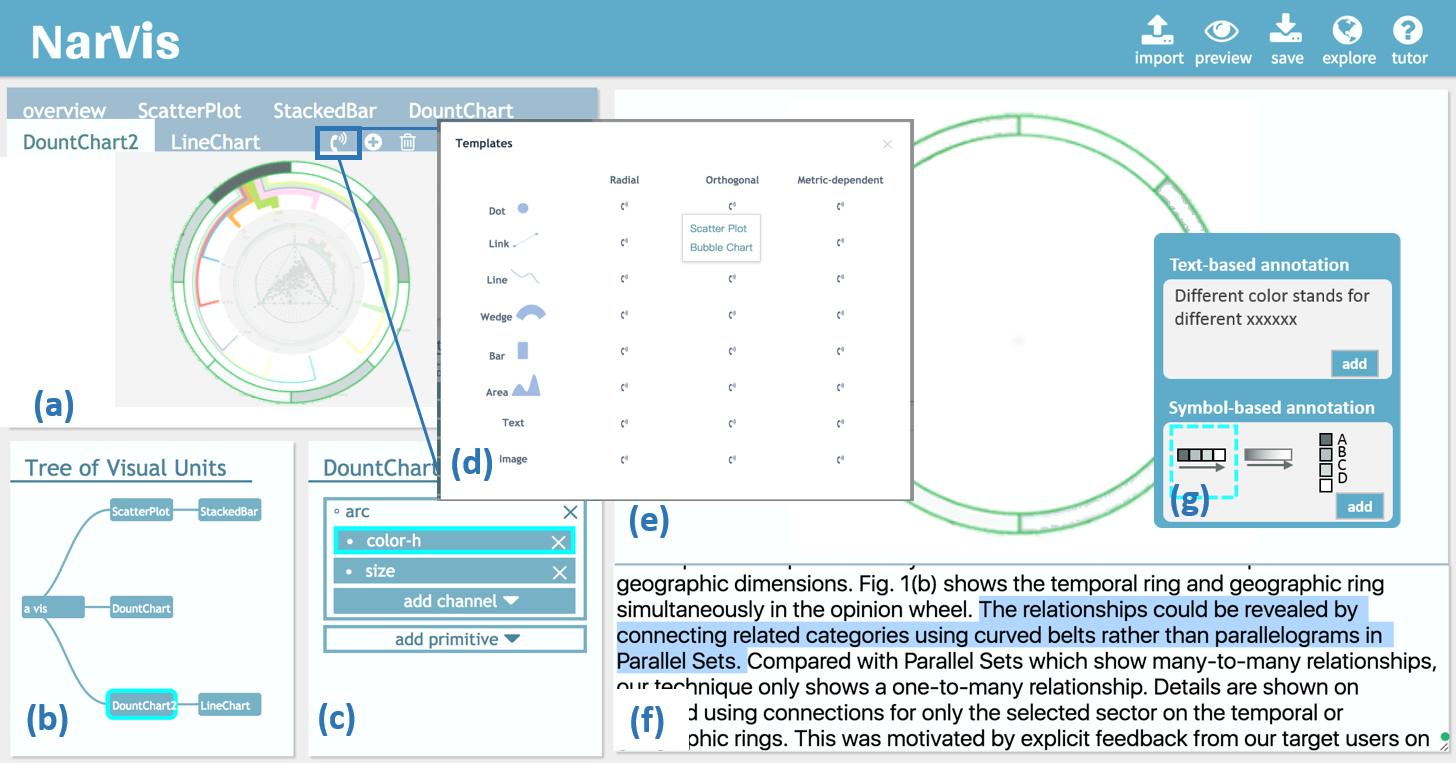
\includegraphics[width=\columnwidth]{interface}
 \caption{Annotated screenshot of the interface of Narvis: a) Source Panel, b) Tree Panel, c) Unit Panel, d) the library of templates, e) Edit Panel, f) text area where the related sentence is highlighted from input textual description, g) a floating annotation window that offers options for adding annotation}
 \label{fig:interface}
\end{figure}


\begin{figure}
 \centering 
 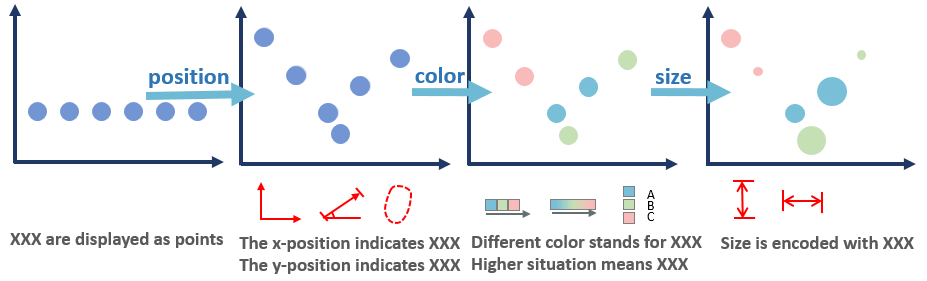
\includegraphics[width=\columnwidth]{tempelate}
 \caption{Demonstration of the template for bubble chart, which is composed of series of slides(top), symbol-based annotation for each visual channel (middle), and text-based annotation for each visual channel(bottom). }
 \label{fig:template}
\end{figure}


\subsection{Phase2: Authoring}
In the Authoring Phase, editors craft an introduction slideshow by constructing built-in blocks called templates in Narvis. We first explain how we design and organize the templates in Narvis, then demonstrate the workflow of this phase, which includes three steps, i.e., invoking templates, organizing templates and modifying templates, as illustrated in Figure~\ref{fig:overview}. 

% We introduce three panels in this phase acting as three steps in the workflow to allow editors  
\subsubsection{A Library of Templates}
We propose a library of templates for the narrative explanation of a visualization. A template is a set of slides that intends to introduce an visual unit. Since an advanced visualization design is the assembly of miscellaneous visual units, such templates can achieve a high level of efficiency for the explanation of a visualization (DA.1). Furthermore, to adapt to various usage scenarios, Narvis allows users to modify and refine templates through rich interactions.

\noindent
\textbf{Types of templates.}
Narvis organize the provided templates with a 8*3 matrix, where the 3 columns stand for 3 construction rules and the 8 rows stand for  8 visual primitives, as shown in Table ~\ref{tab:unit}. Narvis is extensible, we plan to introduce new templates in the future. At the same time, it is desirable to keep the set of supported marks small and well organized, so as to avoid overwhelming users with a cornucopia of confusing options.

\noindent
\textbf{Templates design.}
We apply the analysis and theory model in Section~\ref{analysis} for the design of templates. A template has four core components: 1) a well-considered narrative sequence for visual grammar explanation; 2) exaggeration or suppression of certain visual channels in some slides; 3) a series of narrative techniques such as attention cues, animated transitions, information repetition, to orientate visual attention and facilitate perception (DE.1); 4) Hints for adding annotations (DE.2) in each slide. 

With a visual unit, more specifically, a set of graphic elements, as input, a templates will generate a slideshow and each slide illustrates one visual grammar(DE.1). These slides are sorted based on the narrative sequence we discussed in section 3.3. In each slide, we offer hints to guide the annotation process (DE.2). These hints are sentence with blanks to fill in, heuristic questions, or a list of suggestion symbols. A visual channel is suppressed until its grammar has been explained. For example,in Figure~\ref{fig:template}, before we introduce the visual grammar of color, all the object will be blue. The graphical elements in different slides, which have different visual appearances due to the applied exaggeration or suppression of certain visual channels, are perceptively connected through morphing animation. 

\begin{table}[tb]
  \caption{A summary of animation provided}
  \label{tab:animation}
  \small
  \centering
  \begin{tabular}{p{1cm}|p{0.9cm}|p{0.9cm}|p{0.9cm}|p{1.5cm}|p{0.9cm}}
  \toprule
 \textbf{Animation} &\textbf{Engaging} & \textbf{orientate attention} & \textbf{perception} &\textbf{working scenario} &\textbf{ref} \\ 
  \midrule
  \textbf{Morphing} &\checkmark & \checkmark &\checkmark & grammar of size, grammar of shape & \cite{ruchikachorn_learning_2015, heer_animated_2007} \\ 
  \midrule
  \textbf{Blur} &   &\checkmark  &   & focus+context & \cite{pinto2008selecting}\\ 
 \midrule
  \textbf{Flicker} & & \checkmark &  & focus &\cite{waldner_attractive_2014} \\
  \midrule
  \textbf{Motion} & \checkmark & \checkmark & \checkmark & grammar of position & \cite{huber_visualizing_2005} \\
  \midrule
  \textbf{Zoom-in/out} & \checkmark &\checkmark &  & focus&  \\
  \midrule
  \textbf{Annotation} &  & \checkmark &\checkmark &   textual explain & \cite{segel_narrative_2010 } \\
  \midrule
  \textbf{Fade in/out} &  & \checkmark &  & & \\
  \midrule
  \textbf{Decompose} & \checkmark &  &\checkmark & Show how a visualization is composed by visual units & A novel design by us \\
  \bottomrule

  \end{tabular}
  \vspace{1mm}
\end{table}


\noindent
\textbf{Animation embedded in templates }

Narvis provides 8 types of animation, implement them in templates based on their effects on human attention and perception (DA.1), which has been widely discussed in previous work~\cite{robertson_effectiveness_2008, waldner_attractive_2014, heer_animated_2007}.We also provide a novel decomposition animation, which display how a visualization is decomposed to several visual units. This animation, at the beginning of the introduction slideshow, aims to engage the audience as well as to help them get a sense of overview.(DA.6)
Animation is a double-edge sword, which brings both benefits and pitfalls. We are not discuss its effects here but leave it to the judgement of editors by giving them the freedom to remove it.


\subsubsection{Invoking Templates} 

After graphical elements are extracted and clustered based on visual representation, each cluster appears as a tabbed panel in the \textit{Source Panel} (Figure ~\ref{fig:interface}(a)). 

Editors can switch between these tabbed panels, add or delete graphical elements in each panel, making sure that 1) all the graphical elements of the same visual unit is in the same panel 2) every graphical element belongs to one and only panel. Then, for each visual unit, editors call a template from all the templates provided by Narvis (see in Figure~\ref{fig:interface}(d)). 

The relationship between graphical elements and templates is similar to the one between data and function. Templates contain a set of operations to produce a sequence of slides from the input graphical elements. For example, in Figure~\ref{fig:template}, the ``scatter plot'' templates modify the appearance of the input picture and outputs 4 slides that describe different visual grammars. 

\subsubsection{Organizing Templates} 
Once invoked, a template will show on the \textit{Tree Panel}(Figure ~\ref{fig:interface}(b)) as a tree node. 
By dragging and dropping these nodes, editors organize the structure of the tree diagram, which reflects the relationship between visual units and determines the narrative sequence of the slideshow. This tree diagram will be automatically inserted in the generated slideshow, demonstrating the overall structure to the audience (DA. 6). 

\subsubsection{Modifying Templates} 
% \textbf{\textit{ Unit Panel \& Editor panel}: personalized modification}
% but it also allow the users high flexibity to modify these temples, thus guaranteeing the expressiveness of this system. 
Narvis provides templates to generate slideshows with high efficiency. 
It also supports flexible modification of templates for expressiveness.
Editors can edit a template in the \textit{Unit Panel}(Figure~\ref{fig:interface}(c)) by selecting a node on the \textit{Tree Panel}. In each template, all possible visual grammar are enumerated. Editors can delete unused one themselves, instead of adding the ones used, thus eliminating the unconscious omission of crucial information (DA.5).
It also recommends a narrative sequence of visual grammars, based on the metrics we mentioned in Section~\ref{relationship} (DA.2). 
In the \textit{Editor Panel} (Figure~\ref{fig:interface}(e)), with the hints from Narvis, editors add annotations to facilitate graph and chart comprehension. For each slide, which is defaulted to explain one visual grammar in our templates, Narvis offers questions or sentence with blank for adding text-based annotation and a list of suggested design options for symbol-based annotation (DE. 2) that can be added into the slide by a simple one-click (DE.1), as show in Figure~\ref{fig:interface}(g).



\begin{figure}
 \centering 
 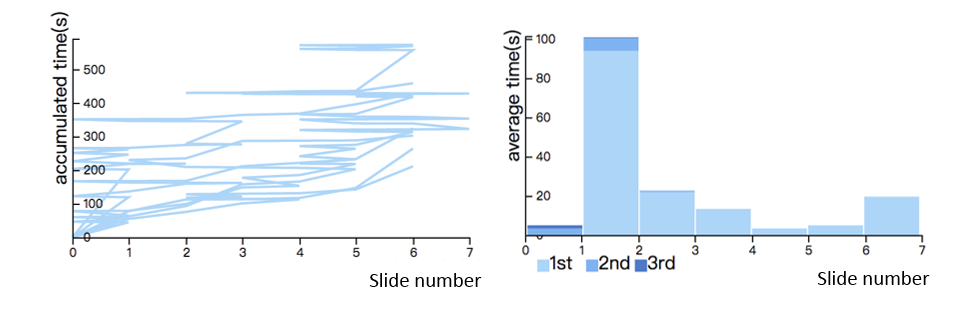
\includegraphics[width=\columnwidth]{feedback}
 \caption{The click stream data of one slideshow visualized as a line chart (left) and a stacked bar chart(right)}
 \label{fig:feedback}
\end{figure}


\subsection{Phase3: Viewing}
The slideshow produced by editors will then be watched by the audiences. By clicking the ``explore'' icon on the right top, audience will be directed to a new window, where Narvis exhibit all the slideshows produced and uploaded.
Audience can choose one slideshow for watching, click buttons to move forward or backward to view all the slides it contains. Their click activity will be recorded automatically by Narvis for the analysis of their watching behavior. 

These clickstream data will be visualized in the form of a stacked bar chart and a line chart (see in Figure~\ref{fig:feedback}).  
The x axis represents the slide's number in both charts. In line chart, the y axis represents the accumulated watching times, and each line refers to the watching behavior of one individual audience. In the bar chart, the y axis represents the average watching time of all users for a certain slide. Each bar is splited into colored bar segments. The bottom bar segment represents the time audience spent the first time for watching this slide, if they go back and watch this slide for a second time, a bar segment with darker color will be placed on the top of the previous one, and so on. 

The line chart emphasizes on the watching behavior of every individual while the bar chart focus on the description of every single slide. \notsure{do i need this?For example, in Figure~\ref{fig:feedback}, the line chart indicates that some audiences go back frequently while other audience go through all the slides sequentially. The bar chart indicates that it is the second slide that audience spent relatively longer time to read. Even though the going back behavior is frequent, the time people spent for it is little.} 
With the help of these two charts, the editor is able observe how the audiences watch his slideshow and generates ideas for later revision (DE.3). 

%\subsection{Iterative Design}
%To investigate the usability of Narvis, we invited 4 UGs from diverse backgrounds to watch an introduction slideshow produced with Narvis. 
%Based on their feedback, we iterate over the design of Narvis as follow:
%
%\subsubsection{An Compulsory Introduction}
%In the initial design, an introduction slideshow is purely the combination of templates. In other words, it just explains each visual units after displaying an overview of the visualization. However, the participants complained that they were less motivated to learn a visual design without an awareness of the background. Questions like, \textit{what's the motivation of this visual design}, \textit{what's the dataset}, and \textit{what kinds of problems it can solve} need to be answered before the introduction of this visual design. Thus, we added a compulsory introduction slide at the beginning of each slideshow, which is displayed as a root node of the tree diagram in \textit{Tree Panel}. This slide contains questions that guide the editors to give a brief description of the background.
%\subsubsection{Different Levels of Detail}
%While 3 UGs appreciate this detailed introduction slideshow, and consider the animation applied as engaging and enjoyable. Another UG, who has taken a data visualization course before and is familiar with some visualization designs, thought some slides and animation are redundant. 
%Thus, we offer 3 levels of details which the audience can choose from. The detailed one displays all the animation, the normal ones skip the animation for some simple visual grammar such as color and size, and the abstract one discards all animation and put the annotation for color and size in one slide
 
 
 \begin{figure*}
 \centering % avoid the use of \begin{center}...\end{center} and use \centering instead (more compact)
 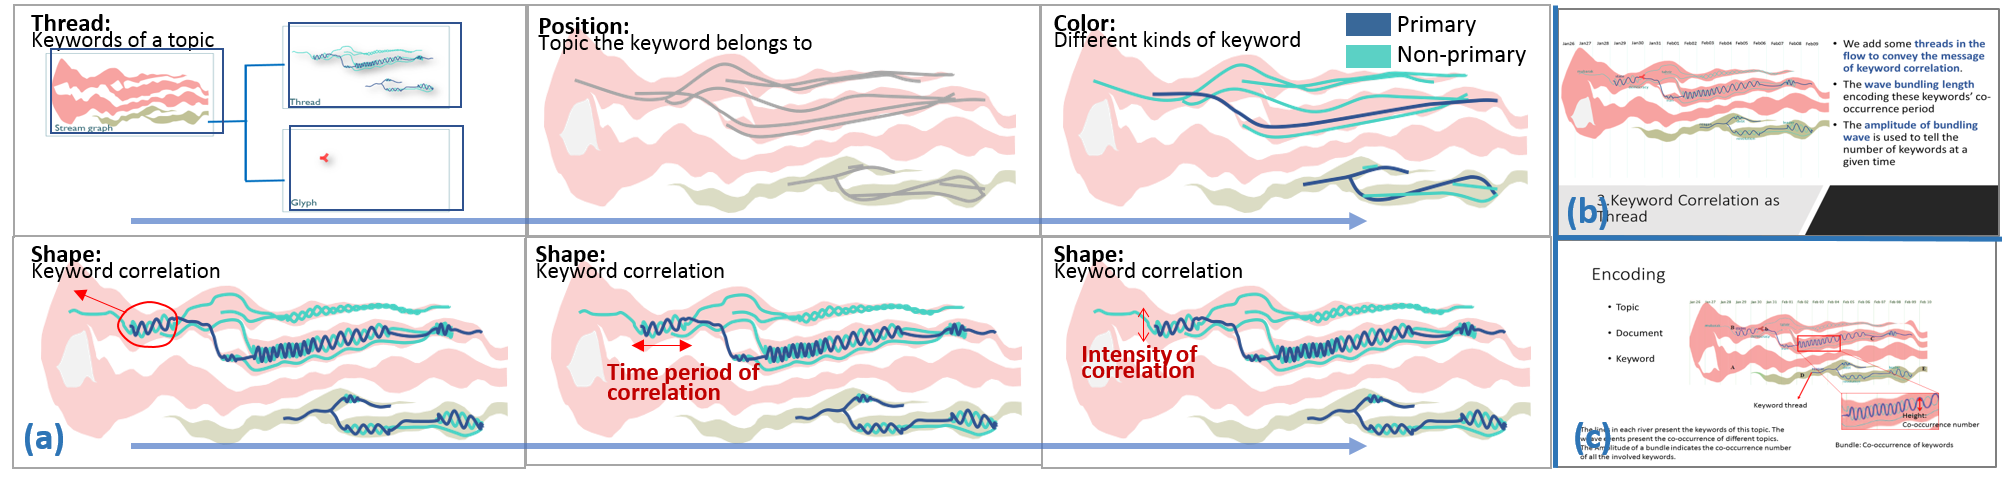
\includegraphics[width=\linewidth]{user_study}
 \caption{The slideshows produced by (a)Narvis and (b),(c)Power Point to introduce a visual unit, thread, in \textit{TextFlow}\cite{cui_textflow:_2011}. Note that (b) and (c) both miss the visual grammar of thread color and (c) forgets to mention the visual grammar of wave bundling length. }
 \label{fig:user_study}
\end{figure*}
 
\subsection{A Working Scenario}
Jessica has extensive experience in the field of data visualization, and has implement a visual analytics tool in a review service website based on the design of OpinionSeer\cite{wu_opinionseer:_2010}, which has five visual units as demonstrated in Figure~\ref{fig:hierarchic}. To help audience better understand this design, she needs to publish a tutorial accompanied with it.
First, she loads the screen-shot of her system, as well a textual description, into Narvis.
After a few seconds, the system automatically extracts the graphical elements. Jessica first adds five tabbed panels (see in Figure~\ref{fig:interface}(a)), since she identifies five different visual units in OpinionSeer. At each panel, where the uploaded image shows with half-transparency as background, Jessica adds graphical elements by clicking it. As in Figure~\ref{fig:interface}(a)), the ``geometry ring'' is added to a tabbed panel and highlighted. Note that Narvis pre clusters some graphical elements to convenient the users. For example, all the dots in ``scatter plot'' will be highlighted just by clicking on one dot. 

After some editing, each tabbed panel includes all graphics elements belonging to one visual unit. Now, she chooses templates for each visual unit. 
She first choose a visual unit by clicking its tab, then clicks the ``phone'' icon. A table Figure~\ref{fig:interface}(d) jumps up, which categorizes all the templates as the 8*3 table we described in Section~\ref{compositions}. For example, when Jessica clicks on the (2,1) cell, a dropdown list that contains two templates, the templates for bubble chart and scatter plot, will appear.  

One by one, Jessica invokes 5 templates, all then show as tree nodes in \textit{Tree Panel} as children of the ``a vis'' node. Jessica reorganizes the structure of the tree diagram (see in Figure~\ref{fig:interface}(b)) by dragging and dropping based on her understanding of this visual design. 

Moreover, Jessica edits the narrative templates based on her design. 
% In the templates, we enumerate all the possible visual encodings. 
She goes through all five templates in the \textit{Unit Panel} by clicking the corresponding node in \textit{Tree Panel}, and deletes the visual channels with no encodings, such as the size in the template of scatter plot. 

Jessica further adds annotations at each slide with the help from an annotation window(see in Figure~\ref{fig:interface}(g)). This annotation windows offers some design options for adding text-based annotation as well as symbol based annotation.  The text area Figure~\ref{fig:interface}(f) also offer hints for the addition of annotation by highlight the corresponding textual description. 
% When adding annotation to a certain channel, the related text will highlight in the text area, aiming to offer a better user experience.   


To refine the readability of the tutorial, Jessica asks several friends, who have little experience in data visualization, to watch the tutorial before release. Narvis collects their viewing behavior from click activities, generates statistics results, and visualize it in the form of a stacked bar chart and a line chart (Figure~\ref{fig:feedback}). From these two charts, Jessica finds out that people spent significantly longer time on reading the 4th slide, which points out that information in this slide is not clear or too complicated. Jessica then revises her slideshow accordingly. 




\section{Evaluation}
\subsection{Participants}
There are two kinds of participants, editors and audiences,  in our user study.\par 
\textbf{Editors: }they are experts in data visualization. They will be divided into two groups and exploit either Narvis or PowerPoint to generate a slide show that explains a visualization design.  \par
\textbf{Audience: }they have no previous experience in data visualization. A questionnaire is conducted to investigate their knowledge about visualization. They will review the slide show produced by the experts, rank it, give subjective comments, and answer a series of questions to check their understanding of this visualization.\par
For editors, we have 4 postgraduate students, aging between 22-30, and all of them have more than one year experience in data visualization.\par
For audiences, we have 20 under graduate students, whose majors vary from business to biology. According to the questionnaire, none of them have accessed advanced data visualization before. Only 13\% students know the tree map, and none can give a accurate explanation of theme river with topic splitting and merging.  \par
\subsection{Material}
We extract the visualization design and the corresponding literature description from  a visualization design paper by Cui et al\cite{cui_textflow:_2011} \par
We choose this visual design based on two considerations. First, it's not too difficult for a laymen but still a novel design that requires extra effect to clarify its encoding scheme.
Second, it is a typical abstract data visualization that is fully consist of graphical element, not involving 3D image or real world image such like satellite map, which is beyond the coverage of our edge detection algorithm. \par
This visualization design is aimed at providing a better understanding about topic evolution in large text collections. It conveys multiple level results of topic evolution analysis: a set of topics
with splitting/merging relationships among each other, which encodes a series of topic flows, a set of critical events, which encode glyphs, and the keyword correlations, which encode threads.  \par
\subsection{Procedure}
\subsubsection{Producing}
We run a two-hour long sessions, which is consist of 3 phases: (1)\textit{learn visualization}, (2)\textit{idea generation and sketch}, (3)\textit{authoring}.\par
In the \textit{learn visualization} phase, participants read the literature description we extract from the paper, which is two-page long and describes the visual design with diagrams. This phase ends when the participants report the experimenters that they finished reading and understand this visual design. This phase takes about 15min, since all the participants are experts in data visualization and familiar with reading such papers.\par
In the \textit{idea generation and sketch} phase, participants are asked to sketch ideas for introducing \textit{TextFlow} to general public. They are encouraged to give considerations to (1) knowledge base of the audience, (2) information complexity of different visual encodings, (3) attention cues to orientate audience's attention. Participants are asked to think aloud and experimenters are present in the room to observe. \par
In the \textit{authoring} phase, participants implement the ideas in their sketch as many as possible in a one-hour-long session. Participants in control group use Power Point, a presentation making tool that all the participants are familiar with. In experimental group, before authoring, experimenters demonstrate the capacity of Narvis through an automatic step by step tutorial included in Narvis, using intro.js. This training lasts about 15 min and is not counted in the one-hour authoring session. Participants are also allowed to ask additional questions in the authoring phase.\par
\subsubsection{Reviewing and feedback}
We ask a group of 20 volunteers to evaluate the quality of the generated slide show. We conduct a questionnaire in advance to make sure that they all have no experience or knowledge in advanced data visualization. In a one-hour session, they are asked to view, comment, and rate these slide shows. They also answer a series of questions to check their understanding of the visualization design. \par 
We record video during this session with the participants permission. For participants who review the slide show generated by Narvis, their click activity will be recorded automatically and they can make comments on the slides. These click stream data, as well as the comments stream, will be used to generate a report, which will then send to its editor. \par
To conclude the user study, the experimenters conduct an interview with the participants about their authoring experience, the issues they encountered, if there are any, and the feedback report Narvis generated. \par
\subsection{Results}
We analyzed the following material: 1) video and notes that the experimenters took during the user study session, which the participants consented to. 2) the slides and the sketch created by participants, 3) the interview with the editor participants, 4) the ranking, comments, answers, click stream data from the reviewer participants. While analyzing, we focus on extracting information on the following aspects: 1)
\subsubsection{}
\subsubsection{}
xuke\par
reading 15min\par
draft 5min \par
making slides 40min \par
qiaomu\par
reading 14min\par
draft 5min\par
making slide 40min\par
\subsubsection{Generated slideshow}
\subsubsection{Authoring experience}
\section{Limitation and Discussion}

Results of our study indicate that editors could make slideshow more efficiently with Narvis than with professional software. In addition, audience report that the perceived quality of slideshow generated with Narvis is higher than those created by editors from scratch. However, we identify four limitations existed in Narvis.

First, the library of templates cannot cover all innovative designs. In current prototype, we allow users to extend existing templates to alleviate this issue. 
% To deal with emerging designs, we plan to adopt more custom-defined templates by creating open platform that supports template sharing and downloading in future research. 
% Second, to decompose visualization precisely, users are required to import images with high resolution, which cannot be guaranteed. 
Second, the results of visualization decomposition highly depend on the quality of imported images. We plan to design more robust algorithm to tackle input with various resolution.
Third, interactive features are important and commonly-seen in modern visualization. However, Narvis is limited to static visual design. We plan to investigate narrative introduction of interactions in future research. The fourth limitation of our study is the evaluation. \siwei{I do not know what is our limitations in evaluation. Involve small number of editors? Or audience? The evaluation of quality of slideshow is limited? Our system is only compared to ppt? We try small number of designs? }

It worth noting that we propose a model for narrative presentation of data visualization. The model can be generalized to create other forms of presentation, such as narrative posters and data videos. \siwei{more generalization is better}


% We are not pretending that Narvis are exclusive for all types of visualization design. However, by allowing users a high flexibility to create and edit templates, we believe its coverage  will quickly broaden as more and more users contribute their own templates to our library. \par
% Metaphor for aesthetic purpose.
% Our algorithm, not applicable for 3d rendering picture. 
% In our model, we focus on statistic image and leave dynamic interaction at this time point, which is an important feature for advanced data visualization design. 


\section{Conclusion and Future Work}
We have presented Narvis, an authoring tool to generate slideshow for explaining visual designs. We developed Narvis based on our close collaboration with two editors and seven audience. \siwei{I am not sure about the logic workflow. Have you decided whether the tasks drive our model and system, or the tasks and model drives the system?}

In future work, we envision two main research directions. First, with the popularity of visualization toolkits, such as D3 \siwei{cite d3 paper}, an increasing number of visual designs are deployed online. To support a border usage scenario, we plan to equip Narvis with the ability to parse and analyze online visualizations. 
Second, we aim at iterative refinement of templates based on click behaviors of audience. Click behavior of audience is valuable for editors to improve and edit their slideshows.  
It will be great if Narvis can give suggestions to editors for revision of slideshow. 


%% if specified like this the section will be committed in review mode



%\bibliographystyle{abbrv}
\bibliographystyle{abbrv-doi}
%\bibliographystyle{abbrv-doi-narrow}
%\bibliographystyle{abbrv-doi-hyperref}
%\bibliographystyle{abbrv-doi-hyperref-narrow}

\bibliography{template}
\end{document}

